%!TEX root = ../main.tex
\section{Embedded Design}\label{sec:Embedded_Design}
\label{sec:emb}
An embedded system is needed to handle a wide range of task. 
It is a requirement for the project that the Zybo board should be used as the embedded system in the project.
The'Zybo board features a Zynq Z-7010 chip from Xilinx, which has an integrated dual-core ARM Cortex-A9 processor and a Xilinx 7-series field programmable gate array (FPGA).
The Zybo board itself consists among other of several buttons, switches, LEDs and connections for USB, Ethernet, HDMI and several PMOD connectors. 
Furtheron the FPGA part will be referred to as the Programmable Logic (PL) and the ARM processor as the Processing System (PS). 


\subsection{Functionality}
An analysis of the complete system yielded the functionalities listed below for the Zybo board. 

\begin{itemize}
\item Digital inputs and outputs
\item Generating PWM
\item Measuring voltage output from LEM sensors and foot pedal
\todo[inline]{Thomas: it is a voltage being measured, but we are indirectly measuring a current?}
\item UART communication with external PC
\item Control algorithms for dq-control
\item Read position from encoder
\item SPI communication as master
\end{itemize}

As can be seen on the list there are multiple different tasks that needs to be handled. 
By looking at them it can be seen that optimally they should be run at different speeds.
The PWM switching frequency should be 20kHz as described in section ????.
\todo[inline]{Thomas: Section that describes pwm switching losses?}
As this is quite fast it should be handled in the PL part of the Zynq chip. 
The rest can be handled on the PS part. 
In order to utilize that some tasks needs to be run at lower frequencies it was choosen to use khaOS which is a Run To Comple Scheduler (RTCS) system made by Karsten Holm Andersen.
\todo[inline]{Thomas: Are there any papers on khaOS that we could reference?}
Using an RTCS makes it easy to schedule tasks to run at different frequencies. 
As an RTCS has no way to preempt tasks it leaves much responsibility to the programmer in order to preserve the real time performance of the system.
When the software is finished tests should be performed to ensure  the real time performance.
khaOS was chosen before other RTCS as the group had knowledge about the system from an Embedded Systems course.

\subsection{Architecture}
The software functionalities was grouped into tasks based on functionality and desired frequency.
A task diagram of the complete system on the Zybo can be seen in figure \ref{fig:task_diagram}.


%\begin{figure}[!h]
%  \includestandalone[width=\textwidth]{graphics/taskdiagram}
%  \caption[Task diagram]{Task diagram showing software tasks as green circles, shared variables as yellow boxes, IP cores as blue boxes, I/O periphirals as limegreen boxes, external signals as orange boxes and external components in red. The PS and PL areas are marked accordingly and arrows show the data and signal direction.}
%  \label{fig:task_diagram }
%\end{figure}

\begin{figure}[!h]
  \includegraphics[width=\textwidth]{graphics/taskdiagram}
  \caption[Task diagram]{Task diagram showing software tasks as green circles, shared variables as yellow boxes, IP cores as blue boxes, I/O periphirals as limegreen boxes, external signals as orange boxes and external components as red boxes. The PS and PL areas are marked accordingly and arrows show the data and signal direction. $C_p$ denotes various controller parameters.}
  \label{fig:task_diagram}
\end{figure}

As can be seen various signals are coming from the outside world through the PL into the PS.
All tasks, IP cores and I/O periphirals will be desribed in the coming sections.

\subsubsection{Three phase PWM generator}
The PWM generator is placed in the PL and is developed using Xilinx System Generator in Matlab Simulink.
The PWM generator is made to have an adjustable frequency and dutycycle.
It was choosen to make a center aligned PWM generator as this introduces less harmonic distortion than edge aligned PWM \cite{power_switching_converters}. 
Furthermore center aligned PWM also produces a symmetrical PWM signal, with a defined midpoint in the PWM-wave where the current can be sampled correctly.
The high limit for the counter can be calculated for a given frequency, $f$, by the following:
$$H = L + \frac{f_{Zybo}}{f\cdot 2}$$
Where H is the high limit, L is the low limit and $f_{zybo}$ is the AXI-clock frequency. 
The PWM counter system can be seen in figure \ref{fig:pwm_counter}.
The counter block will count up or down depending on the input. 
The output from the counter value will go into to two compare blocks along with the high and low limits.
The compare blocks will produce a high signal when the counter value is equal to the high and low limit respectively.
These signals are then fed to a an m-code blocks which contains a simple state machine which determines if the counter should count up or down.
\begin{figure}[!h]
	\centering
	\includegraphics[width=0.8\linewidth]{graphics/counter}
	\caption[Block diagram of counter in PWM generator.]{Simulink block diagram of the counter in the PWM generator.}
	\label{fig:pwm_counter}
\end{figure}
The counter out signal can be seen in figure \ref{fig:pwm_graph}.
The counter signal is then fed into a PWM mechanism shown in figure \ref{fig:pwm}. 
The dutycycle is given to the PWM generator in the datatype u32, an integer type and therefore the dutycycle is given in a range of 0 to 1000, giving a resolution of 0.1\%.
The switching limit will be calculated from the following:
$$l = (1 - \frac{d}{1000}) \cdot r$$
Where l is the switching limit, d is the dutycycle in the range 0 - 1000 and r is the counter range.
A register will then make sure that the switching limit is only passed on when the counter is at its lowest.
It is important to do so as otherwise the dutycycle can be corrupted.
The compare block will make the PWM signal by comparing the switcing limit to the counter value.
The counter signal and output of the PWM generator can be seen in figure \ref{fig:pwm_graph}.
As the PWM generator should be able to do three independent PWM signal there are three of the systems shown in figure \ref{fig:pwm}, one for each phase.

\begin{figure}[!h]
	\centering
	\includegraphics[width=1\linewidth]{graphics/pwm_system}
	\caption[Block diagram of PWM generator.]{Simulink block diagram of the PWM mechanism in the PWM generator.}
	\label{fig:pwm}
\end{figure}

\begin{figure}[!h]
	\begin{center}
		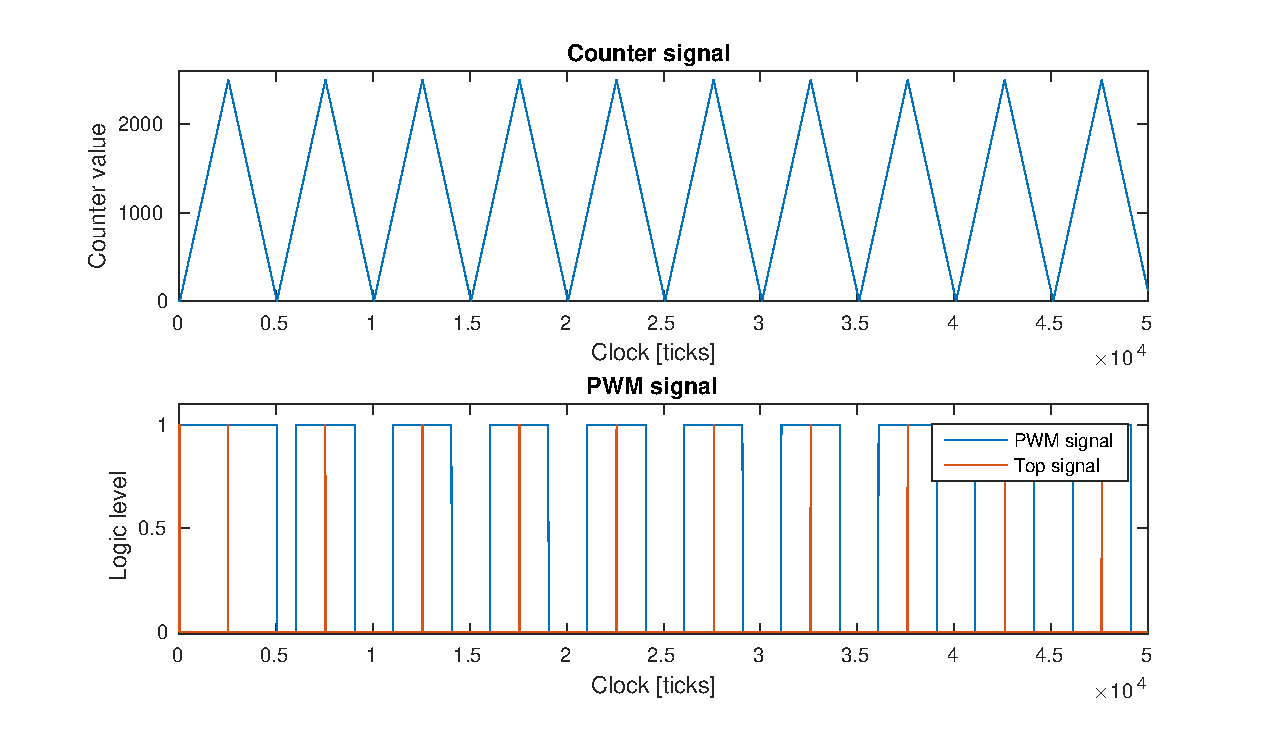
\includegraphics[width=\linewidth]{graphics/pwm_plot}
		\caption{Counter and PWM signal.}
		\label{fig:pwm_graph}
	\end{center}
\end{figure}


\subsubsection{Interface task}
The interface task has to read external signals, output digital signals and control the other tasks.
The task needs to update the enable variable that the controller and PWM task reads.
The basic funcionality of the interface task can be seen in the flowchart of figure \ref{fig:interface}.

%\begin{figure}[!h]
%	\centering
%	\includegraphics[width=0.7\linewidth]{graphics/interface_task}
%	\caption[Block diagram of PWM generator.]{Simulink block diagram of the counter in the PWM generator.}
%	\label{fig:interface}
%\end{figure}

\begin{figure}[!h]
	\centering
	\includestandalone[width=0.5\textwidth]{graphics/interface_flow}
	\caption[Interface task.]{Flow chart illustrating the basic funtionality of the interface task.}
	\label{fig:interface}
\end{figure}
\todo[inline]{Is the inrush relay explained somewhere?? -MIkkel}

At startup the interface task needs to turn on the inrush relay for a certain time.
Afterwards the main relay needs to be turned on and the inrush relay is turned off after some time to be sure that the main relay is conducting.
Then the task will read all signals from the the digital board and if they are all good the global enable variable will be changed to high.
If one or more of the drive signals indicate a fault, the task will change the enable variable to low.

Alongside the functionality of figure \ref{fig:interface} the interface will act as master for the two UART tasks.
This enables the setting of values within the system as well as potentially reading the current status of the system.
All communication through the UART interface is done through the \texttt{rx\_buffer} and \texttt{tx\_buffer} arrays shown in listing \ref{lis:uartvars}.
Currently three parameters can be set within the system:
\begin{itemize}
	\item \texttt{kp/ki}: These are the values of the PI controller used.
	\item \texttt{qmax}: The limit of the current that the controller is allowed to set as reference. 
\end{itemize}
Setting any of the above is done by:
\begin{center}
\texttt{set <parameter> <value>}
\end{center}
As can be seen in listing \ref{lis:cutcommand} the command is split into parts using \texttt{strtok()}.
This is a non-reentrant function that will return all the characters until the first appearance of delimiter.
Every consecutive call to the function with \texttt{NULL} as the first parameter will continue the search through the same array.
With the command split into tokens it is parsed using a simple if-structure, comparing each argument in the command using \texttt{strcmp()} until a value can be set.

\begin{lstlisting}[captionpos=b,style=customCpp, caption={Something clever!.THOMASSSS!}, label=lis:cutcommand, escapeinside={(*@}{@*)}]
if(rx_flag)
{
  char* cmd = strtok(rx_buffer, DELIMITER);
  char* var = strtok(NULL, DELIMITER);
  char* val = strtok(NULL, DELIMITER);
  
  if(!strcmp(cmd,"set"))
  {
    if(!strcmp(var,"kp"))
    {
      scanf(val, "%f", &kp);
      sprintf(tx_buffer, "kp was set: %f", kp);
      tx_flag = true;
      tx_tail = strlen(tx_buffer);
    }
  	
(*@\makebox[.25\linewidth][c]{$\smash{\vdots}$}@*)
  
  }
  rx_flag = false;
  rx_tail = 0x00;
}
\end{lstlisting}

Once the value is set a message is returned to the user, informing of the successful setting.
\texttt{rx\_flag} is cleared and the buffer is emptied by setting \texttt{rx\_tail} to zero.

\todo[inline]{Thomas: Not sure the lines below are relevant, but i felt like writing it...}
The system is made with expandability in mind, currently only a \texttt{set} command is implemented.
This could easily be extended to a \texttt{read} or perhaps a \texttt{shutdown} command.

\subsubsection{Controller task}
\begin{figure}[!h]
	\centering
	\includestandalone[width=0.9\textwidth]{graphics/tikz/Block_diagram1tikz}
%		\includegr%aphics[width=0.9\linewidth,trim=3cm 15cm 0 2cm]{graphics/controller_tasktikz}
	\caption[Block diagram of controller task.]{Block diagram showing the functionality of the controller task.}
	\label{fig:controller_task}
\end{figure}

The basic functionality of the controller task can be seen in figure \ref{fig:controller_task}.
The task polls data from the ADC in order to get the raw data for $I_a$, $I_b$ and the foot pedal.
The raw data from the ADC is then calculated into voltages and the two currents are calculated based by the equation:
\begin{equation}
	 I = \frac{V_{measured}}{R_m} \cdot NS
\end{equation}
$I_c$ is calculated based on the assumption that the three currents form a balanced three phase system.
The resistance of the foot pedal potentiometer is calculated from the measured voltage and equation \ref{eq:pedal_back_calc}.

$I_a$, $I_b$, $I_c$ and $\theta$ are then used to perform a Clarke Park transformation and obtaining the values of $I_d$ and $I_q$. 

$I_d$ and $I_q$ should be controlled towards a setpoint by two seperate controllers.
The setpoint for $I_d$ is 0 as will be explained later?? .
\todo[inline]{Where?} 
The setpoint, $q_{set}$, for $I_q$ should be related to the maximum allowed current, $q_{max}$, and the position of the foot pedal in percent, $pedal_\%$:
\begin{equation}
	q_{set} = pedal_\% \cdot q_{max}
\end{equation}
It was choosen to use two PI controllers as will be described in section \ref{sec:controller_design}.
The code for one of the controllers can be seen in listing \ref{lis:controller_code}.
As can been seen in line 2 trapezoidal integration is used. 
Lines 4-8 performs anti windup and lines 9-14 calculates the output if enable is high and performs integrator reset if low.

\begin{lstlisting}[captionpos=b,style=customCpp, caption={[C code constituting a PI controller.]C code constituting a PI controller with trapezoidal integration, anti windup and integrator reset.}, label=lis:controller_code]
d_error = d_set - I_d_measured;
d_integral = d_integral + (d_previous_error + d_error)*0.5*dt;

if(d_integral > MAX_TOTAL_OUTPUT){
	d_integral = MAX_TOTAL_OUTPUT;
}else if (d_integral < -MAX_TOTAL_OUTPUT){
	d_integral = -MAX_TOTAL_OUTPUT;
}
if(enable){
	d_output = kp * d_error + ki * d_integral;
}else{
	d_output = 0;
	d_integral = 0;
}
d_previous_error = d_error;

\end{lstlisting}
Afterwards $d_{output}$ and $q_{output}$ are 
Afterwards the output values are downscaled if they exceed the maximum limits.
The code for downscaling can be seen in \ref{lis:saturation}.

\begin{lstlisting}[captionpos=b,style=customCpp, caption={[C code for downscaling.]C code for detecting and downscaling output values that exceed the maximum limits.}, label=lis:saturation]
total_output_magnitude = sqrt(d_output*d_output + q_output*q_output);

if(total_output_magnitude > MAX_TOTAL_OUTPUT){
	d_output = (d_output* MAX_TOTAL_OUTPUT)/total_output_magnitude;
	q_output = (q_output* MAX_TOTAL_OUTPUT)/total_output_magnitude;
}
\end{lstlisting}

\subsubsection{PWM task}
\todo[inline]{do I need code here ? - Mikkel}
The PWM tasks basic functionality can be seen in the block diagram of figure \ref{fig:pwm_task}.
The PWM task is a seperate task from the controller task as it might be preferrable to have the two tasks run at different frequencies.
The task reads the rotor position from the encoder and access the global variables $d_{output}$ and $q_{output}$. 
It uses this information to perform inverse Clarke Park transformation.
Afterwards third harmonic injection is performed and if the values are higher or lower than the maximum bounds they are saturated.
The global enable variable is checked and passed to the physcial enable pin.


\begin{figure}[!h]
	\centering
%	\includegraphics[width=0.9\linewidth,trim=2cm 17cm 0cm 4cm]{graphics/pwm_tasktikz}
  	\includegraphics[width=\textwidth]{graphics/PwmTask2}
	\caption[Block diagram of PWM task.]{Block diagram showing the functionality of the PWM task.}
	\label{fig:pwm_task}
\end{figure}

\todo[inline]{Where should we talk about the concept of dq and the meaning of it? -MIkkel}
\todo[inline]{Third harmonic injection and why? -MIkkel}



\subsubsection{ADC}
The Zynq chip contains a dual 12-bit, 1 Mega sample per second (MSPS) Analog-to-Digital Converter (ADC) \cite{adc}.
The ADC is utilized through the XADC Wizard in Vivado. 
The ADC measures the difference between differential analog input pins $V_p$ and $V_n$.
The IP core is configured to use AXI4LITE connection, simultaneous selection, unipolar mode and event mode.
Simultaneous selection mode is used as it allows simultaneous sampling on the dual ADC. 
When using simultaneous sampling the phase relationship is preserved.
When unipolar mode is enabled the input range between $V_p$ and $V_n$ is 1 \si{\volt} and the input voltage must always be positive.
Setting the ADC in event mode, means that the ADC will only sample when there is a rising edge on its CONVST pin. 
The CONVST pin is connected to the top signal of the PWM generator meaning that the ADC will sample in the center of the PWM pulse.
This is done to sample the current correctly. 
Channels 6 and 14 are paired together in simultaneous mode, meaning that they will be sampled simultaneous.
Therefore the outputs from the two LEM sensors will be connected to these. 
The torque pedal signal will be routed to channel 7 which will be sampled after channel 6 and 14.
The top signal from the PWM generator will start the sampling and therefore it will also set the sampling frequency.
As the PWM frequency is 20 \si{\kilo\hertz} the ADC sampling frequency will be so as well.

\subsubsection{UART RX/TX}
In order to facilitate communication between the Zybo board and a PC, a small UART connection is established.
The connection consists of two tasks, UART\_RX and UART\_TX.
They handle receiving and transmitting, respectively.
As shown in listing \ref{lis:uartvars} each of the tasks are given a buffer, a flag and a tail variable.

\begin{lstlisting}[captionpos=b,style=customCpp, caption={UART\_RX/TX buffers and variables.}, label=lis:uartvars]
char rx_buffer[0xff];
char tx_buffer[0xff];
bool rx_flag = false, tx_flag = false;
uint8_t rx_tail = 0x00, tx_tail = 0x00;
\end{lstlisting}

\begin{lstlisting}[captionpos=b,style=customCpp, caption={UART\_RX task.}, label=lis:uartrx]
void uart_rx_task()
{
  if (XUartPs_IsReceiveData(UART_BASEADDR))
  {
    rx_buffer[rx_tail] = XUartPs_ReadReg(UART_BASEADDR, XUARTPS_FIFO_OFFSET);
    rx_tail++;
  }
  if(rx_buffer[rx_tail-1] == '\r')
  {
    rx_flag = true;
  }
  _wait(MILLI_SEC(1));
}
\end{lstlisting}

Looking at listing \ref{lis:uartrx} the function of these in the UART\_RX task can be seen.
If there is data on the line it is pushed onto the \texttt{rx\_buffer} and \texttt{rx\_tail} is incremented.
This is to keep track of the number of characters that have been received.
Finally, if the last character received is a carriage return, the \texttt{rx\_flag} is set high.
This indicates to the interface task that a full command has been received and is ready for execution.
Listing \ref{lis:uarttx} shows the UART\_TX task.
Every time it is run it will check \texttt{tx\_flag}.
If \texttt{tx\_flag} is high, this indicates that data has been put into the \texttt{tx\_buffer}.
All \texttt{tx\_tail} characters in the buffer are transmitted character by character.
Hereafter \texttt{tx\_buffer} is "emptied" by setting \texttt{tx\_tail} to zero and \texttt{tx\_flag} is set low to indicate that transmission is complete.
\begin{lstlisting}[captionpos=b,style=customCpp, caption={UART\_TX task.}, label=lis:uarttx] 
void uart_tx_task()
{
  if(tx_flag)
  {
    uint8_t i;
    for(i = 0; i < tx_tail; i++)
    {
      xil_printf("%c",tx_buffer[i]);
    }
    tx_tail = 0x00;
    tx_flag = false;
  }
  _wait(MILLI_SEC(250));
}
\end{lstlisting}

\subsection{Encoder}
The Zybo board needs to interface the RMB28MD encoder that is mounted on the motor.
The RMB28MD is an absolute encoder with sine/cosine, SSI and incremental output. 
It was choosen to use the SSI output as an IP core reading the position by SSI communication was made available by the supervisors of the group.
Reading the position throug SSI yields a resolution of 8bit per mechanical revolution. 
The physical RMB28MD encoder signals are interfaced by an IP Core..
The IP core outputs a clock to the RMB28MD chip and reads data from a datapin. 
It then makes the data available on the AXI4LITE bus, where it can be read from software by the PWM task. 

\subsection{SPI communication}

\todo[inline]{Thomas: I haven't described our timing issues, it seemed a better thing to do it in this section?}
\begin{figure}[!h]
	\centering
		\includegraphics[width=1\linewidth]{graphics/spi_timing}
	\caption[SPI timing requirements.]{SPI timing requirements.From datasheet? How to cite?}
	\label{fig:spi_timing}
\end{figure}

As described earlier the Zybo board will need to set certain parameters on the DRV8301 chip using SPI communication. 
The Zynq chip has two SPI controllers in the PS area of the chip, which can be setup to communicate with external devices.
By investigation the Zynq datasheet \cite{zynq_reference} it  was found that it was not possible to configure the SPI controller to meet the requirements of the DRV8301. 
More specifically it was not possible to configure the clock signal to go low for a minimum of 40 \si{\nano\second} \cite{DRV8301}, before Slave Select goes low. 

Two solutions were found to this problem:
\begin{enumerate}
	\item To develop a simple SPI driver in VHDL or System Generator to send 16bit according to the SPI requirements of the DRV8301.
	\item To use the SPI controller in PS of the Zynq and delay the Slave Select signal physically.
\end{enumerate}
It was found that the most correct solution to the problem would be to develop a SPI driver, but due to time considarations it was choosen to use the SPI controller of the Zynq.

SPI 1 on the Zynq was used as it can be ported to MIO channels 10 to 15, which can be accessed through the PMOD connectors of the Zybo board. 
The SPI controller was initialized in software and was configured to be in master mode, manuel chip select mode and manuel start mode by writing to the configuration register Config\_reg0.
In order to comply with the SPI specifications of the DRV8301 it was configured with the XSPIPS\_CLK\_PHASE\_1\_OPTION in order to make data valid on falling edges of the clock. 
The discharge of a capacitor is utialized to make a delay on the Slave Select signal, by putting a XX capacitor and XX resistor in series with the signal.
The transmission of \texttt{0b0001000000110000} were measured by an oscilloscope and can be seen in figure \ref{fig:spi_graph}.

\begin{figure}[!h]
	\centering
		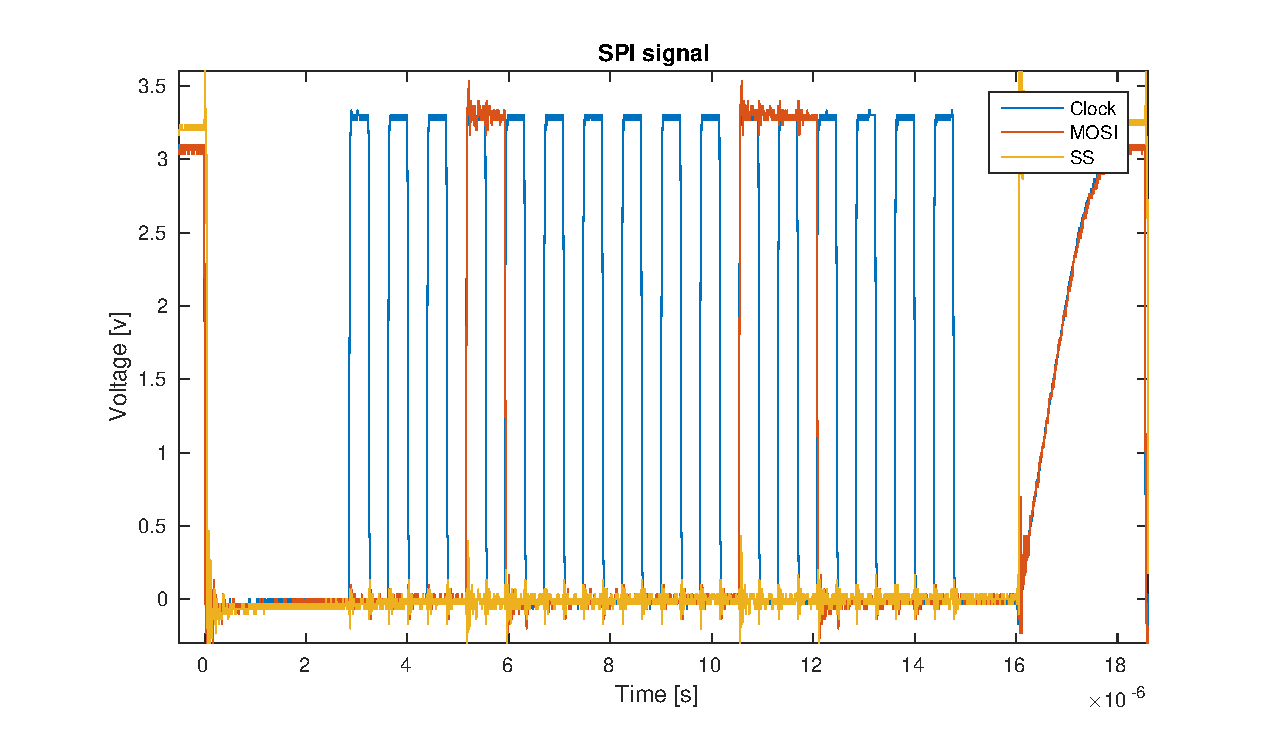
\includegraphics[width=1\linewidth]{graphics/spi}
	\caption[SPI transmission.]{SPI transmission of two data bytes.}
	\label{fig:spi_graph}
\end{figure}


\subsection{Task frequencies}

\subsection{Timing TEST or whatever}

\todo[inline]{Write about the task frequencies}

%\subsection{Conclusion}